\documentclass[a4paper,11pt]{article}
\usepackage[utf8]{inputenc}
\usepackage[italian]{babel}
\usepackage{amsmath}
\usepackage{amsfonts}
\usepackage{amssymb}
\usepackage{physics}
\usepackage{graphicx}
\usepackage{subfig}
\usepackage{hyperref}
\usepackage{parskip}
\usepackage{tabu, wrapfig}
\usepackage{multicol}
\usepackage[italiano, ruled]{algorithm2e}
\usepackage[left=1in, right=1in]{geometry}

\newcommand{\avg}[1]{\langle {#1} \rangle}
\newcommand{\code}[1]{\texttt{#1}}
\newcommand{\chindof}{\chi^2 / \text{ndof}}

\title{Simulazione numerica del modello di Ising 2D}
\author{Rocco Francesco Basta}
\date{}

\begin{document}
	\maketitle
	\section{Introduzione}
		Il modello di Ising 2D consiste in un reticolo di spin, ognuno dei quali può assumere un valore discreto $s_i = \pm 1$ ed interagisce con i suoi primi vicini e, eventualmente, con un campo magnetico esterno.

		L'Hamiltoniana del sistema è data da

		\begin{equation}
			H = -J\sum_{<ij>} s_i s_j - h \sum_i s_i
		\end{equation}

		dove $J > 0$ è la costante di accoppiamento fra primi vicini, mentre $h$ è un campo magnetico esterno.

		Possiamo definire la densità di magnetizzazione $M$, la densità di
		energia $\epsilon$, la suscettività magnetica $\chi$ e il calore
		specifico $C$ del sistema: sia $V$ il volume del reticolo,

		\begin{subequations}
		\begin{multicols}{2}

		\begin{equation}
			M \equiv \frac{1}{V} \sum_i s_i
		\end{equation}
		\begin{equation}
			\epsilon \equiv \frac{E}{V}
		\end{equation}
		
		\begin{equation}
			\chi \equiv \frac{\partial \avg{M}}{\partial h} \propto V ( \avg{M^2} - \avg{M}^2)
		\end{equation}
		\begin{equation}
			C \equiv \frac{\partial \avg{\epsilon}}{\partial T} \propto V (\avg{\epsilon^2} - \avg{\epsilon}^2)
		\end{equation}
		\end{multicols}

		\end{subequations}

		Il modello presenta una transizione di fase del secondo ordine per
		$\beta_c \equiv 1/T_{c} \simeq 0.4407$. Attorno al punto critico, la lunghezza di
		correlazione $\xi$ diverge, e il comportamento del sistema è descritto
		dagli esponenti critici $\alpha, \beta, \gamma, \nu$. Definendo la temperatura ridotta $t \equiv \beta - \beta_c$,

		\begin{subequations}
		\begin{multicols}{2}
		\begin{equation}
			\xi \sim |t|^{-\nu} 
		\end{equation}
		\begin{equation}
			\avg{M} \sim |t|^\beta \quad (T < T_c) 
		\end{equation}
		\begin{equation}
			\chi \sim |t|^{-\gamma}
		\end{equation}
		\begin{equation}
			C \sim |t|^{-\alpha}
		\end{equation}
		\end{multicols}
		\label{eqn:t_scaling}
		\end{subequations}

		Gli esponenti critici sono noti esattamente: $\nu = 1$, $\beta = 1/8$,
		$\gamma = 7/4$, $\alpha = 0$.

		Le simulazioni sono effettuate a volume finito. Di conseguenza, $\avg{M}$ non è un buon parametro d'ordine, perché per simulazioni abbastanza lunghe si deve annullare. Al suo posto, si deve studiare $\avg{|M|}$, e anche $\chi$ va misurata calcolando la varianza di $|M|$.
		
		Per non appesantire la scrittura, d'ora in poi indicheremo semplicemente con $M, \epsilon$ le quantità $\avg{|M|}, \avg{\epsilon}$.
		
		Per volumi finiti, $\xi$ non può divergere e diventa confrontabile
		con $L$. Assumendo che nell'intorno della transizione il sistema perda
		memoria del comportamento microscopico (e quindi della spaziatura del
		reticolo),
		si ottengono delle relazioni di scaling per $M$, $\chi$ e $C$:

		\begin{subequations}
		  \begin{equation}
			\chi(\beta, L) = L^{\gamma/\nu} f_\chi (tL^{1/\nu})
		  \end{equation}
		  \begin{equation}
			C(\beta, L) = L^{\alpha/\nu} f_C (tL^{1/\nu})
		  \end{equation}
		  \begin{equation}
			M(\beta, L) = L^{\beta/\nu} f_M(tL^{1/\nu})
		  \end{equation}
		  \label{eqn:fs_scaling}
		\end{subequations}

	\section{Simulazioni numeriche}

	La transizione è stata studiata attraverso un algoritmo Metropolis locale per
	reticoli di dimensione $N = 20,30,40,50,60$, con $\beta$ compreso tra 0.3 e
	0.505. Per ogni coppia $(N, \beta )$,
	sono state prese $10^{5}$ misure, ognuna ogni spazzata di update, partendo da un reticolo di spin orientati casualmente. 
	
	Il numero di misure scartate per termalizzazione è stato determinato confrontando con simulazioni analoghe fatte partendo da un reticolo di spin paralleli fra loro.

	La simulazione è stata effettuata in assenza di campo magnetico esterno
	($h = 0$), e fissando $J = 1$.

	Gli errori su $\epsilon$ e $M$ sono stati
	stimati attraverso un processo di blocking, mentre gli errori su $\chi$ e $C$ sono stati stimati attraverso un algoritmo Bootstrap.

	Il generatore di numeri casuali utilizzato è \code{RAN2}, tratto dalle \emph{Numerical Recipes for C}.
	
	\subsection{Misure effettuate}
	
	Sono riportati in figura \ref{fig:em_plot} i grafici di $M, \epsilon$ in funzione di $\beta$ ottenuti nelle simulazioni. In figura \ref{fig:chiC_plot} invece è riportato l'andamento di $\chi$ e di $C$.
	
	\begin{figure}[htb]
        \subfloat[$M$]{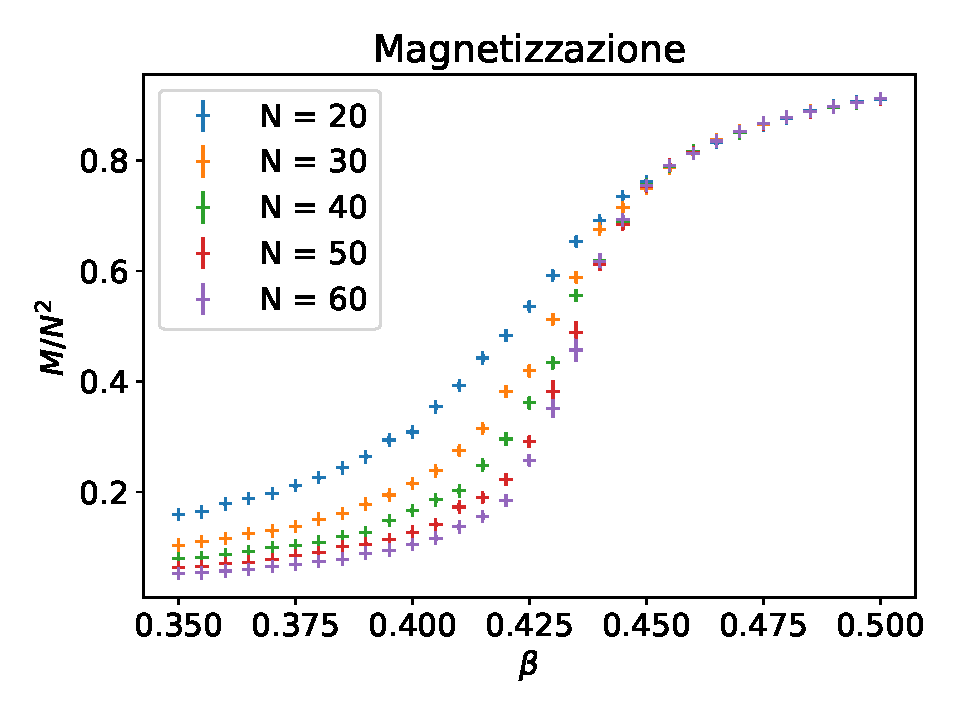
\includegraphics[width=0.5\textwidth]{figure/m_plot.pdf}}
        \subfloat[$\epsilon$]{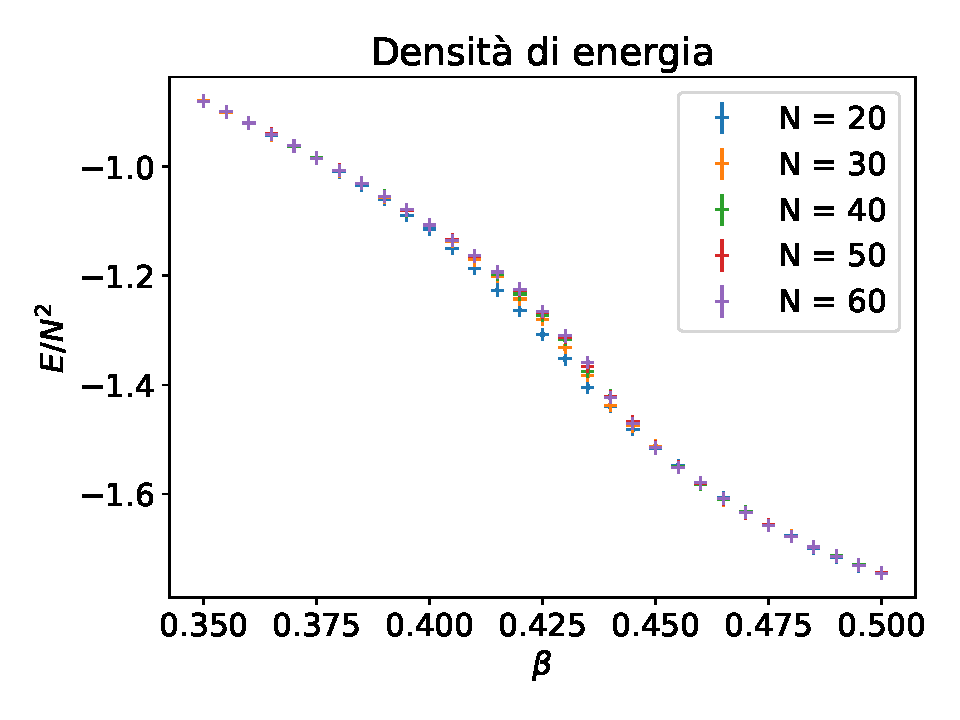
\includegraphics[width=0.5\textwidth]{figure/e_plot.pdf}}
        \caption{Magnetizzazione e densità di energia in funzione di $\beta$.}
        \label{fig:em_plot}
	\end{figure}
	
	\begin{figure}[htb]
        \subfloat[$\chi$]{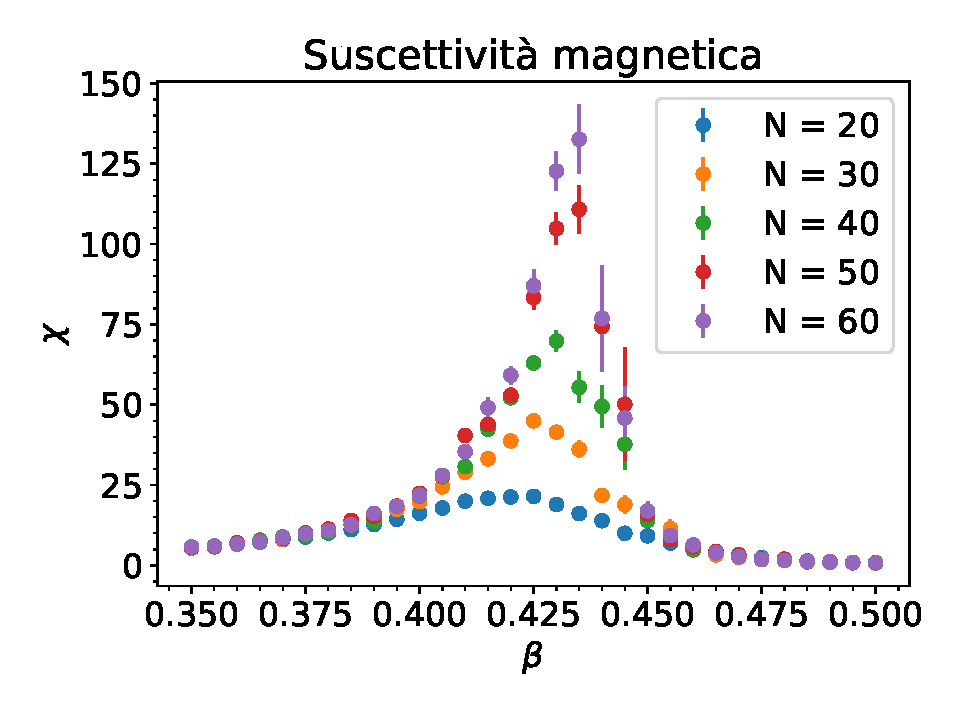
\includegraphics[width=0.5\textwidth]{figure/chi_plot.pdf}}
        \subfloat[$C$]{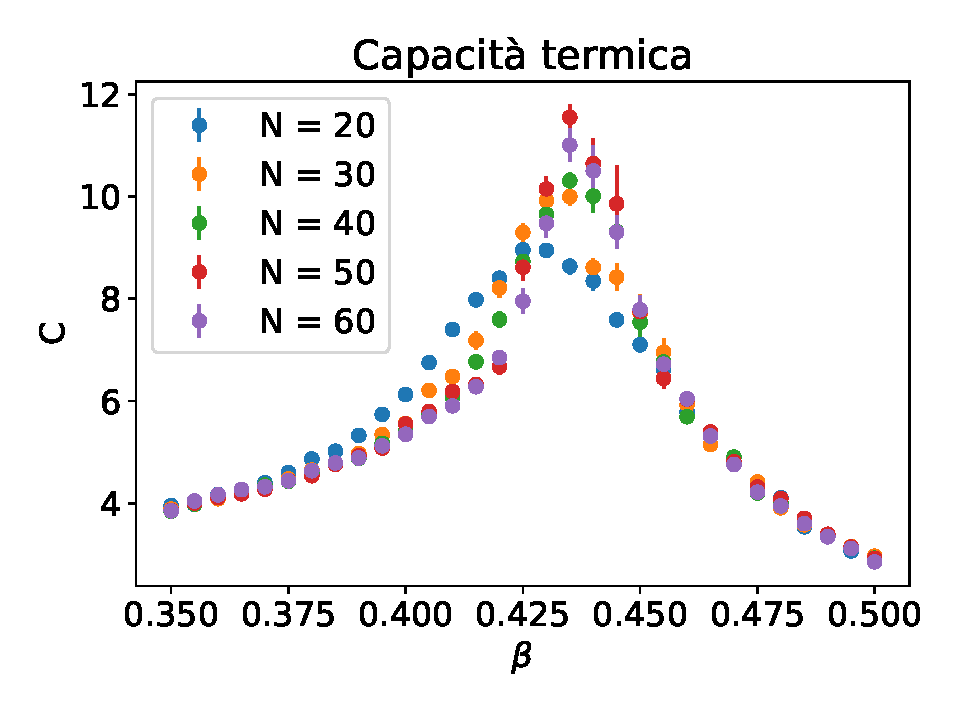
\includegraphics[width=0.5\textwidth]{figure/C_plot.pdf}}
        \caption{Suscettività magnetica e calore specifico in funzione di $\beta$.}
        \label{fig:chiC_plot}
	\end{figure}
	
	Possiamo utilizzare i valori teorici degli indici critici per verificare le relazioni di scaling (eq. \ref{eqn:fs_scaling}). Il risultato è riportato in figura \ref{fig:mchiC_scaling_plot}. Per ottenere il collasso per il calore specifico, è stato necessario sottrarre un termine di fondo che non diverge attorno al punto critico. Per semplicità, questo è stato fatto sottraendo a $C$ il suo massimo, per ogni $N$, prima di applicare la relazione di scaling.
	
	\begin{figure}[htb]
        \subfloat[$M$]{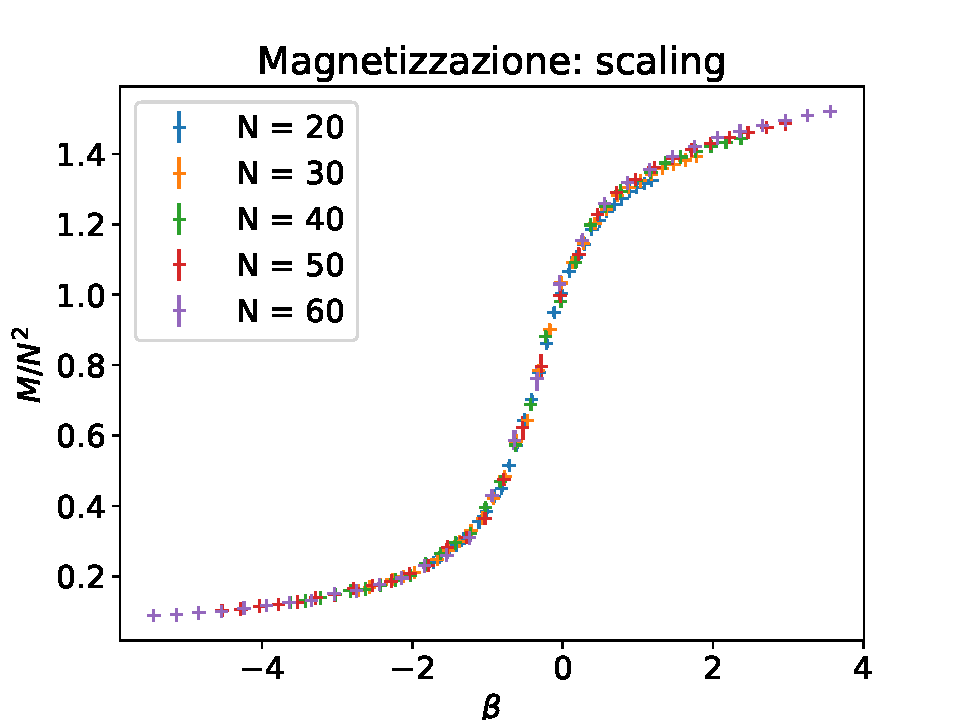
\includegraphics[width=0.5\textwidth]{figure/m_scaling.pdf}}
        \subfloat[$\chi$]{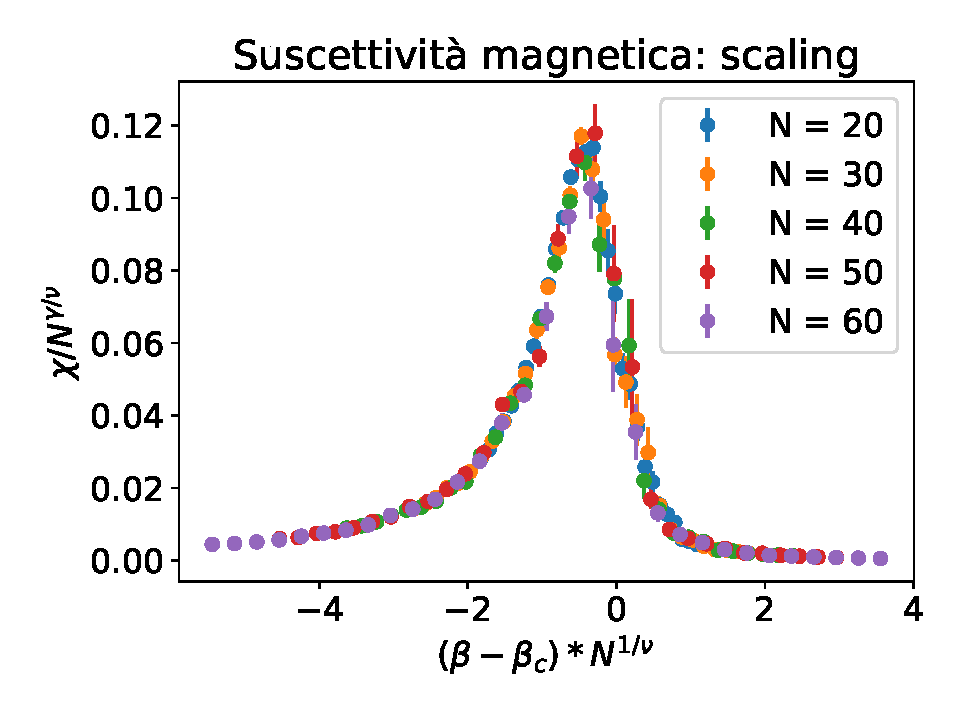
\includegraphics[width=0.5\textwidth]{figure/chi_scaling.pdf}} \\
        \subfloat[$C$]{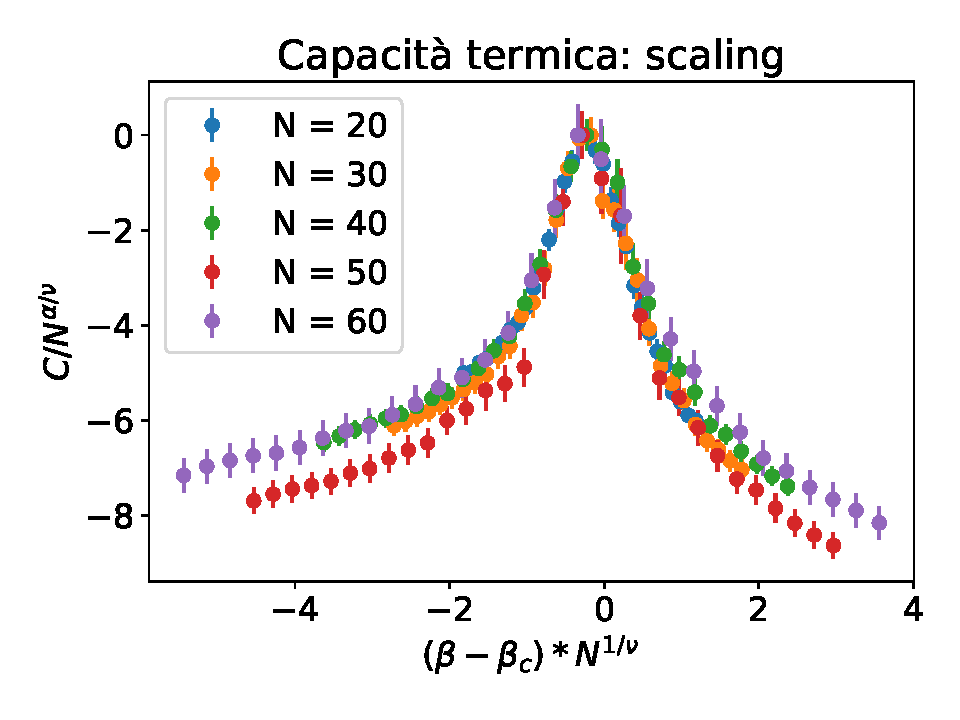
\includegraphics[width=0.5\textwidth]{figure/C_scaling.pdf}}
        \caption{Verifica dello scaling di size finito per $M$, $\chi$, $C$ utilizzando i valori teorici degli indici critici.}
        \label{fig:mchiC_scaling_plot}
	\end{figure}

	
	\subsection{Temperatura critica}
	
    \begin{wraptable}{r}{6cm}
        \centering
        \begin{tabular}{c c} \hline
            N & $\beta_{pc}$ \\ \hline
            20 &     0.4250(25)   \\ 
            30 &     0.4250(25)   \\ 
            40 &     0.4300(25)    \\ 
            50 &     0.4350(25)   \\ 
            60 &     0.4350(25)   \\ \hline
        \end{tabular}
        \caption{Misure di $\beta_{pc} (N)$.}
        \label{tab:bpc_scaling}
        \vspace{5mm}
        \centering
        \begin{tabular}{c | c } \hline
                %$\beta_c$    & x          & corr. & $\chindof$ \\ \hline
                %0.4395(29) & -0.33(9)   & -0.925    & 1.24 \\ \hline
                $\beta_c$   & 0.4395(29) \\
                x           & -0.33(9) \\
                corr.       & -0.925 \\
                $\chindof$  & 1.24 \\ \hline
        \end{tabular}
        \caption{Misura di $\beta_c$ dal fit analitico di $\beta_{pc}(N)$ all'eq. (\ref{eqn:bpc_scaling}).}
        \label{tab:bpc_fit}        
    \end{wraptable}
	
    A N finito, il massimo di $\chi$ non corrisponde a $\beta_c$, ma a un valore inferiore, detto $\beta_{pc}$ ($\beta$ pseudocritico). Lo stesso avviene per $C$, ad una diversa temperatura $\beta'_{pc}$.
    
    Dalle equazioni (\ref{eqn:t_scaling}) e (\ref{eqn:fs_scaling}) è facile dimostrare che $\beta_{pc}$ soddisfa una relazione analoga
    % 
    \begin{equation}
        \beta_{pc} = \beta_c + x N^{-1/\nu}
        \label{eqn:bpc_scaling}
    \end{equation}
    %
    da cui possiamo ricavare $\beta_c$ e $\nu$.
    
    
    
    Alle misure di $\beta_{pc}$ ottenute considerando il massimo della suscettività, è stato associato un errore $\Delta \beta_{pc}$ pari a metà della distanza tra due misure consecutive ($\Delta \beta_{pc} = 0.0025$). Queste misure sono riportate in tabella \ref{tab:bpc_scaling}.
    
    Non è stato possibile effettuare un fit numerico alla funzione (\ref{eqn:bpc_scaling}) lasciando liberi tutti e tre i parametri $\beta_c$, $x$ e $\nu$, per problemi di convergenza del fit.
    
    Tuttavia, un fit con $\nu = 1$ fissato fornisce $\beta_c = 0.4395(29)$, che è compatibile con il valore teorico, con un $\chi^2 / \text{ndof} \simeq 1.24$. Il grafico è riportato nella figura \ref{fig:bpc_fit}, mentre i dettagli del fit sono in tabella \ref{tab:bpc_fit}.
    
    \begin{figure}
        \centering
        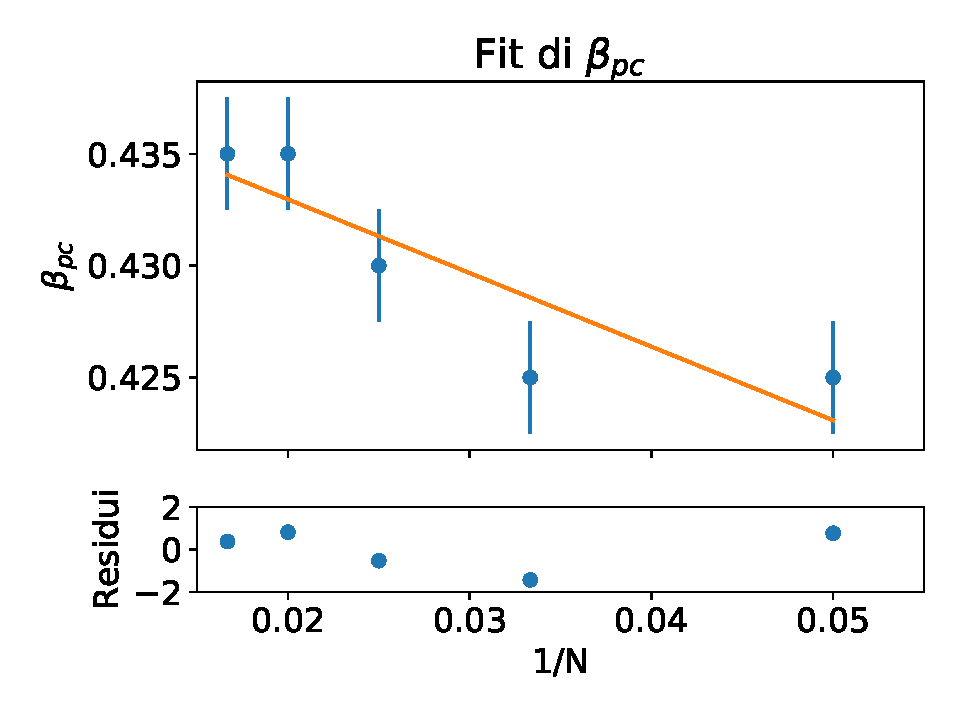
\includegraphics[width=0.7\textwidth]{figure/fit_bpc.pdf}
        \caption{Misura di $\beta_c$ dal fit di $\beta_{pc}(N)$.}
        \label{fig:bpc_fit}
    \end{figure}
    



	
	\subsection{Scaling rispetto alla temperatura}
	
	Si è tentato di estrarre gli indici critici $\alpha, \beta, \gamma$ da un fit analitico di $\chi, C, M$ in funzione di $t$, vicino alla transizione.
	Il fatto che $\alpha = 0$ implica $C \sim \log(t)$ nella regione scalante. I dati sono quindi stati fittati alle equazioni
	
	\begin{subequations}
        \begin{equation}
            \log \chi = - \gamma \log t + c
        \end{equation}
         \begin{equation}
            C = a \log t + c
        \end{equation}  
        \begin{equation}
            \log M = \beta \log t + c
        \end{equation}
	\end{subequations}

	\begin{table}[hbt]
        \centering
        \begin{tabular}{c | c c c c c } \hline 
                                  & $\gamma$  & c    & corr. & $\chindof$ & regione scalante \\ \hline
                $\beta > \beta_c$ & 1.783(53) & -5.31(17)   & -0.996    & 1.77 & $0.01 < |t| < 0.05$ \\
                $\beta < \beta_c$ & 1.743(45) & -2.48(13)   &   -0.997 & 0.76 & $0.03 < |t| < 0.08$ \\ \hline
        \end{tabular}
        \caption{Fit analitico di $\chi$ nella regione scalante.}
        \label{tab:chi_fit}
        \vspace{5mm}
        \centering
        \begin{tabular}{c | c c c c c } \hline 
                                  & a  & b    & corr. & $\chindof$ & regione scalante \\ \hline
                $\beta > \beta_c$ & -2.683(45) & -4.73(14)   & 0.996   & 1.23 & $0.09 < |t| < 0.06$ \\
                $\beta < \beta_c$ & -1.839(40) & -0.49(11)   & 0.995   & 1.34 & $0.03 < |t| < 0.1$ \\ \hline
        \end{tabular}
        \caption{Fit analitico di $C$ nella regione scalante.}
        \label{tab:C_fit}
	\end{table}
	
	I fit sono stati effettuati con le misure ottenute dal reticolo più grande ($N = 60$), e sono stati eseguiti sia per $t > 0$ che per $t < 0$ (tranne nel caso di $M$, perché la relazione di scaling vale solo per $T < T_c$).
	
	I fit per $\chi$ e $C$ sono riportati nelle figure \ref{fig:chi_fit} e \ref{fig:C_fit}. In tabella \ref{tab:chi_fit} sono riportati i valori ottenuti per $\gamma$, insieme al $\chi^2 / \text{ndof}$ e all'intervallo di temperature considerato per il fit. Il risultato è in buon accordo col valore teorico. In tabella \ref{tab:C_fit} sono invece riportati i valori ottenuti dal fit del calore specifico. Anch'esso è in buon accordo con il modello.

	
	\begin{figure}
        \centering
        \subfloat[$\beta > \beta_c$]{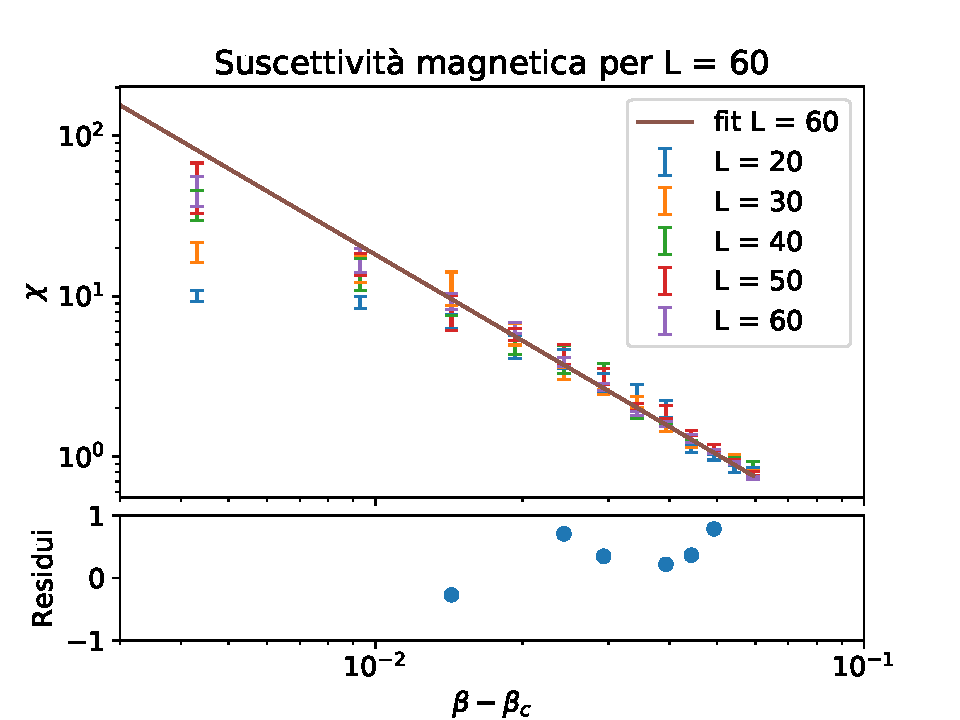
\includegraphics[width=0.5\textwidth]{figure/chi_fit.pdf}}
        \subfloat[$\beta < \beta_c$]{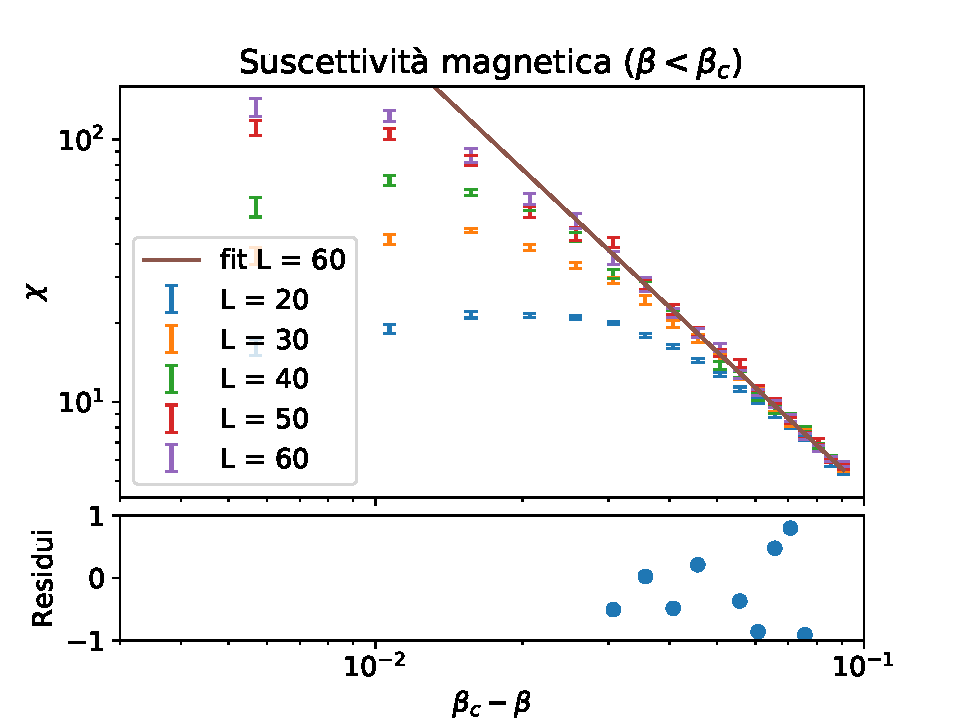
\includegraphics[width=0.5\textwidth]{figure/chi_fit_rev.pdf}}
        \caption{Fit della suscettività magnetica $\chi$ nella regione scalante.}
        \label{fig:chi_fit}
	\end{figure}

	\begin{figure}
        \centering
        \subfloat[$\beta > \beta_c$]{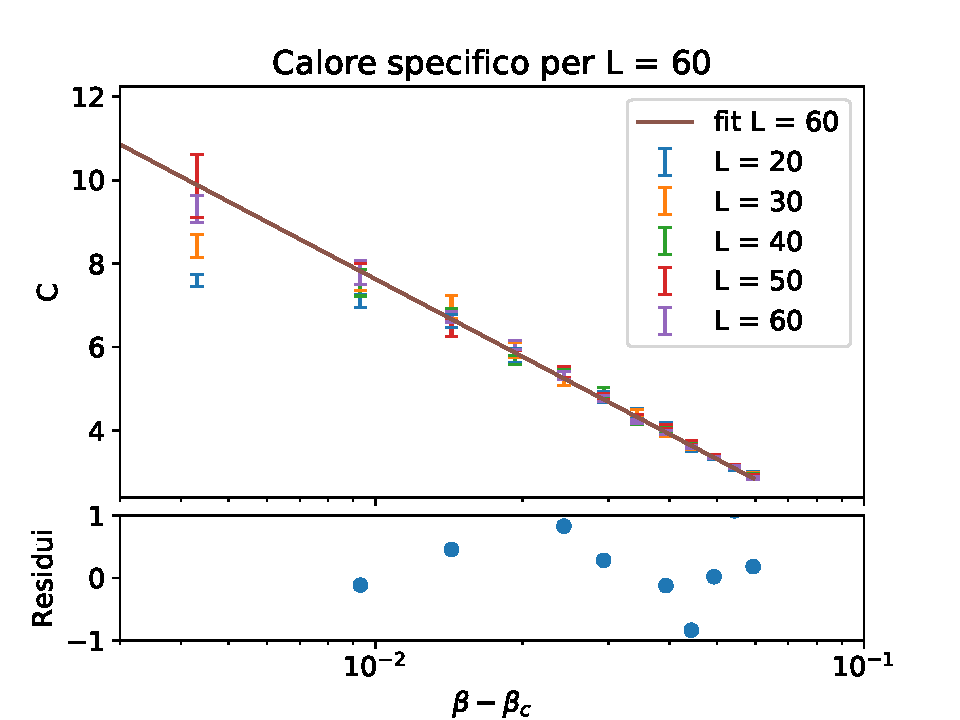
\includegraphics[width=0.5\textwidth]{figure/C_fit.pdf}}
        \subfloat[$\beta < \beta_c$]{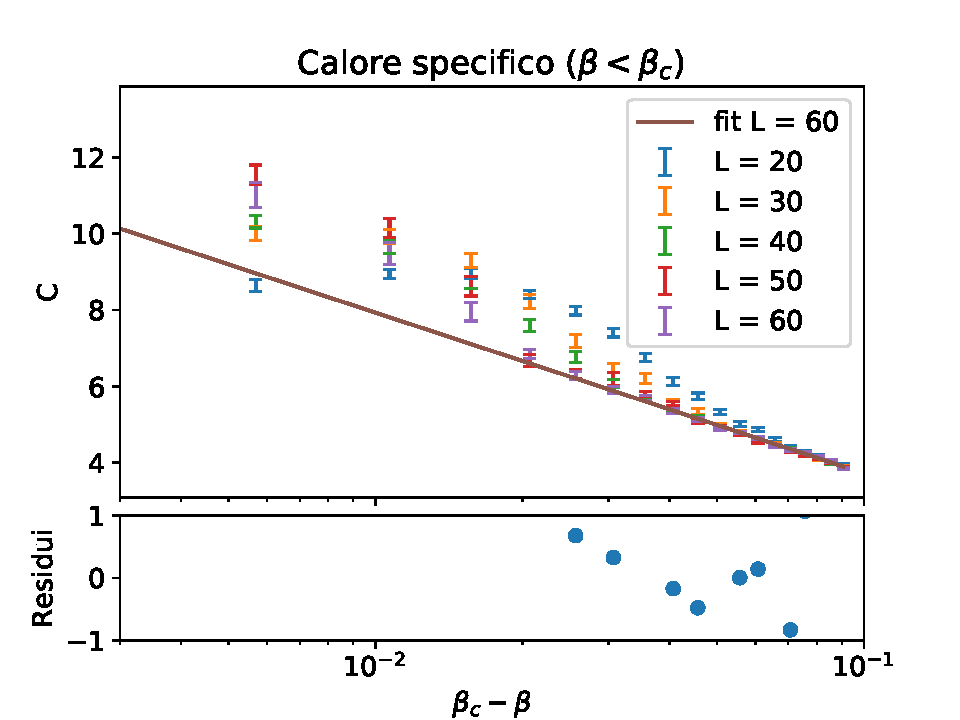
\includegraphics[width=0.5\textwidth]{figure/C_fit_rev.pdf}}
        \caption{Fit del calore specifico $C$ nella regione scalante.}
        \label{fig:C_fit}
	\end{figure}
	
	Il fit di $M$ con questo metodo non ha restituito un valore di $\beta$ compatibile con il valore teorico $\beta = 0.125$. Il risultato, riportato in tabella \ref{tab:M_fit} e in figura \ref{fig:M_fit}, è fuori di più di 10$\sigma$ rispetto al valore teorico. Questo è probabilmente dovuto alla difficoltà di individuare la giusta regione di scaling. L'errore, inoltre, non include il contributo dovuto proprio all'arbitrarietà della scelta della regione in cui eseguire il fit, e quindi è sicuramente sottostimato.
	
	\begin{figure}[htb]
        \centering
        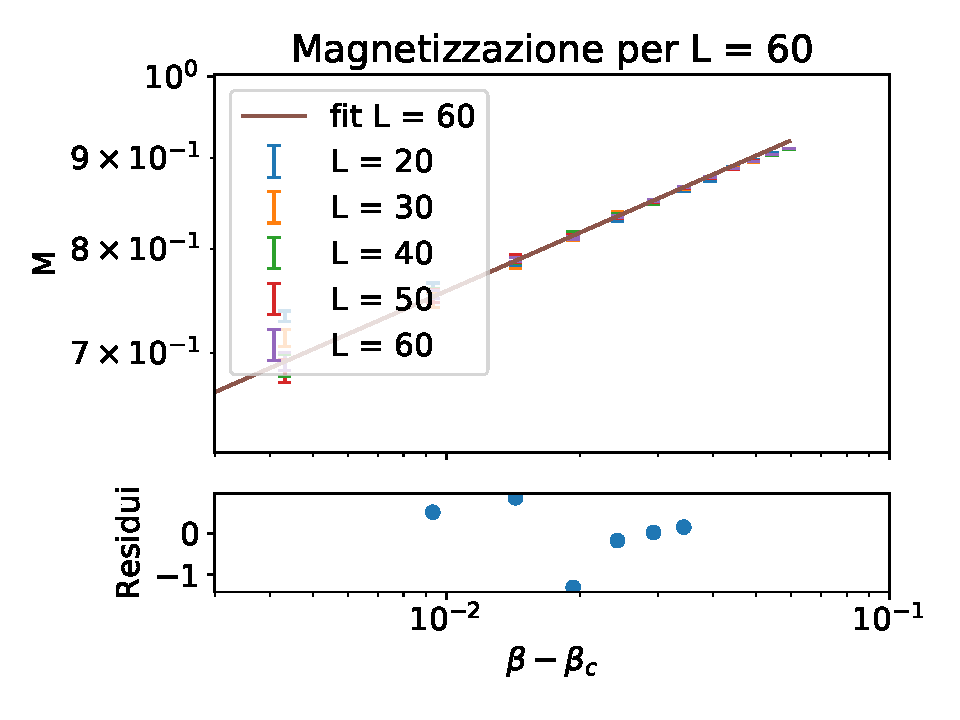
\includegraphics[width=0.7\textwidth]{figure/m_fit.pdf}
        \caption{Fit della magnetizzazione $M$ nella regione scalante.}
        \label{fig:M_fit}
	\end{figure}
	
	\begin{table}[htb]
       \centering
        \begin{tabular}{c c c c c } \hline 
                $\beta$  & c    & corr. & $\chindof$ & regione scalante \\ \hline
                0.1086(18) & 0.223(6)   & 0.998   & 0.699 & $0.008 < |t| < 0.035$ \\ \hline
        \end{tabular}
        \caption{Fit analitico di $C$ nella regione scalante.}
        \label{tab:M_fit}
	\end{table}

	\subsection{Analisi di size finito per $\beta = \beta_c$}
	\begin{wraptable}{r}{6.5cm}
       \centering
        \begin{tabular}{c c c c } \hline 
                $\gamma/\nu$  & c    & corr. & $\chindof$ \\ 
                1.739(31) & -2.57(11)   & 0.993   & 1.67 \\ \hline
                a  & b    & corr. & $\chindof$ \\ 
                2.554(78) & 0.66(27)   & -0.992   & 1.12 \\ \hline
                $-\beta/\nu$  & c    & corr. & $\chindof$ \\ 
                0.1220(39) & -0.002(13)   & 0.992   & 0.68 \\ \hline
        \end{tabular}
        \caption{Fit analitico di $\chi_c(N)$, $C_c(N)$ e $M_c(N)$.}
        \label{tab:fs_fit}
	\end{wraptable}
	Dato il risultato insoddisfacente dell'ultimo fit, si è provato a misurare gli indici critici del modello studiando gli effetti di size finito. Sono state effettuate nuove simulazioni con $\beta = 0.440687 \simeq \beta_c$, N = 20, 25, 30, 25, 40, 45, 50, 55, 60, 65, 70, 80, 90, 100. Per ogni simulazione sono state prese 125000 misure, una ogni 10 spazzate, e il numero di misure scartate per termalizzazione è stato determinato nello stesso modo.
	
	L'idea è di sfruttare le equazioni (\ref{eqn:fs_scaling}) per ottenere da un fit i rapporti $\beta / \nu$, $\alpha / \nu$, $\gamma / \nu$. 

	
	I dati raccolti sono stati quindi fittati con le seguenti funzioni:
    %	
	\begin{subequations}
        \begin{equation}
            \log \chi_c = - \frac{\gamma}{\nu} \log N + c
        \end{equation}
         \begin{equation}
            C_c = a \log N + c
        \end{equation}  
        \begin{equation}
            \log M_c = \frac{\beta}{\nu} \log N + c
        \end{equation}
	\end{subequations}
    %	
	I risultati dei fit sono riportati nelle figure \ref{fig:chi_fs_fit}, \ref{fig:C_fs_fit}, \ref{fig:M_fs_fit} e nella tabella \ref{tab:fs_fit}. In tutti e tre i casi, si ha un ottimo accordo con la previsione teorica. In particolare, la stima di $\beta / \nu$ ottenuta con questo metodo è compatibile con il valore teorico $\beta / \nu = 1/8$, a differenza della stima di $\beta$ ottenuta studiando lo scaling rispetto a $t$.
	
	\begin{figure}[h!]
        \centering
        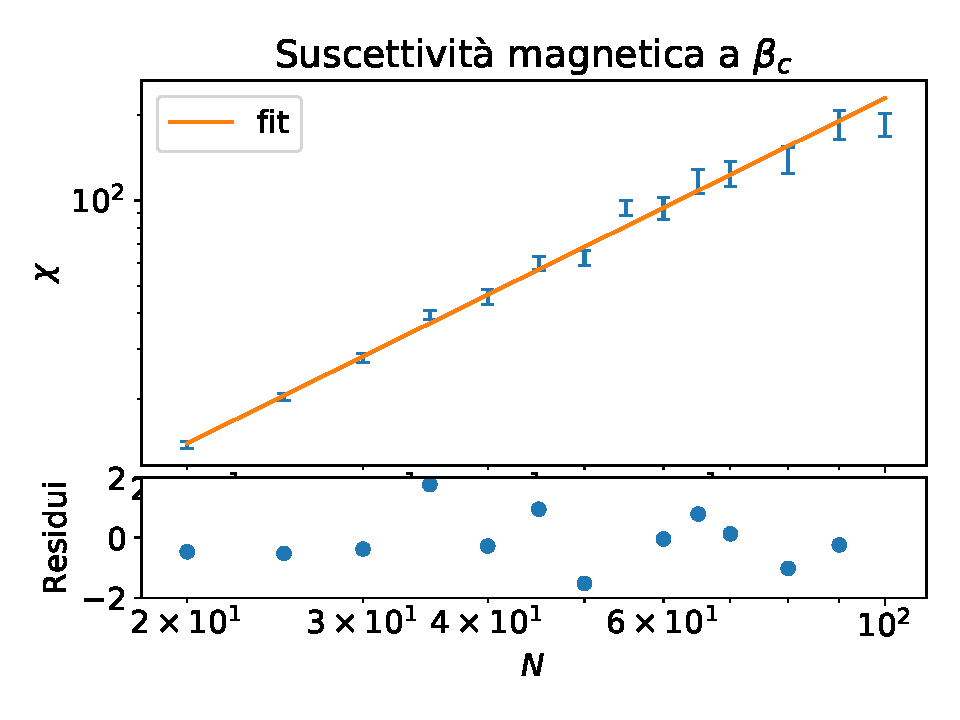
\includegraphics[width=0.7\textwidth]{figure/chi_fs_fit.pdf}
        \caption{Fit analitico di $\chi_c(N)$.}
        \label{fig:chi_fs_fit}
	\end{figure}

	\begin{figure}[h]
        \centering
        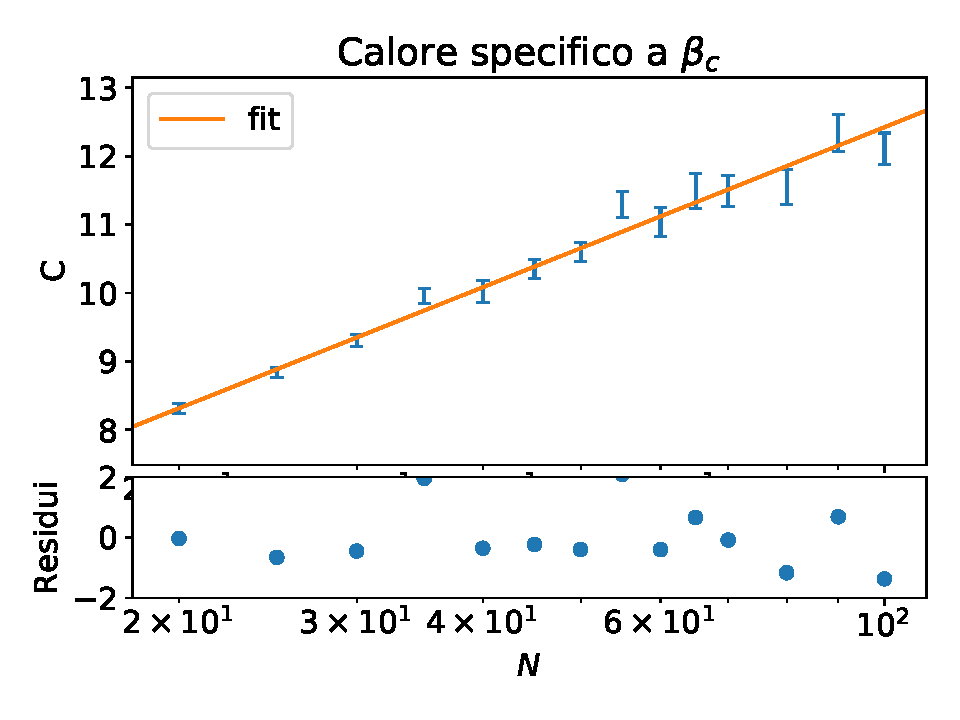
\includegraphics[width=0.7\textwidth]{figure/C_fs_fit.pdf}
        \caption{Fit analitico di $C_c(N)$.}
        \label{fig:C_fs_fit}
	\end{figure}
	
	
	\begin{figure}[h]
        \centering
        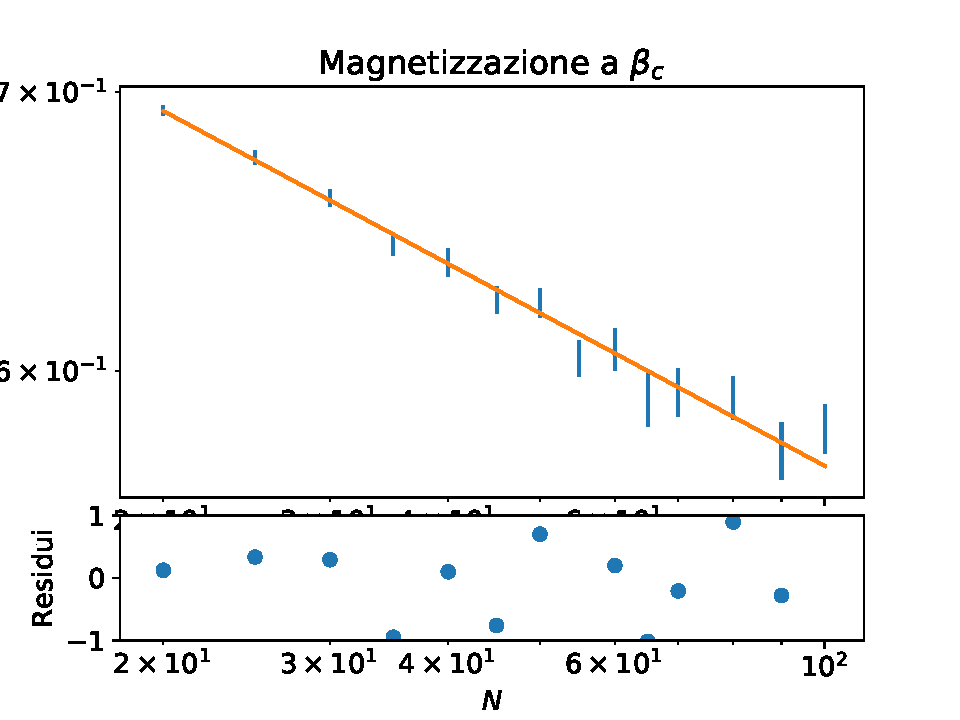
\includegraphics[width=0.7\textwidth]{figure/m_fs_fit.pdf}
        \caption{Fit analitico di $M_c(N)$.}
        \label{fig:M_fs_fit}
	\end{figure}
	
	
	
	
\end{document}
